\section{Related work} \label{releatedWork}
This section covers an overview of the material that is the direct foundation for this research proposal.

\subsection{Inferred model} \label{inferred-model}
The master thesis by Mulders had two significant outcomes. The first is an inferred model module, and the second is the visualisation of the inferred models \cite{thesisMulders}. The visualisation model is a web-based application that shows the inferred model with screenshots and properties. Although the visualisation module becomes required when we want to visualise the result of the change-detection software, it is not necessary to go into depth in this document. This section will discuss what an inferred model is and how they are generated. 

The GUI state was discussed in section \ref{gui-state}. The section ended with the sentence that the universe of states and actions of the SUT's GUI makes up the inferred model. The inferred model is a directed graph showing the GUI-state of the application and the transactions between states. The vertex of the graph represents the GUI-state. Each vertex has a set of incoming and outgoing edges, called the actions. 

Figure \ref{fig:state-model} shows the result of the inferred model in the visualisation module.

\bigskip
\begingroup
\captionsetup{type=figure}
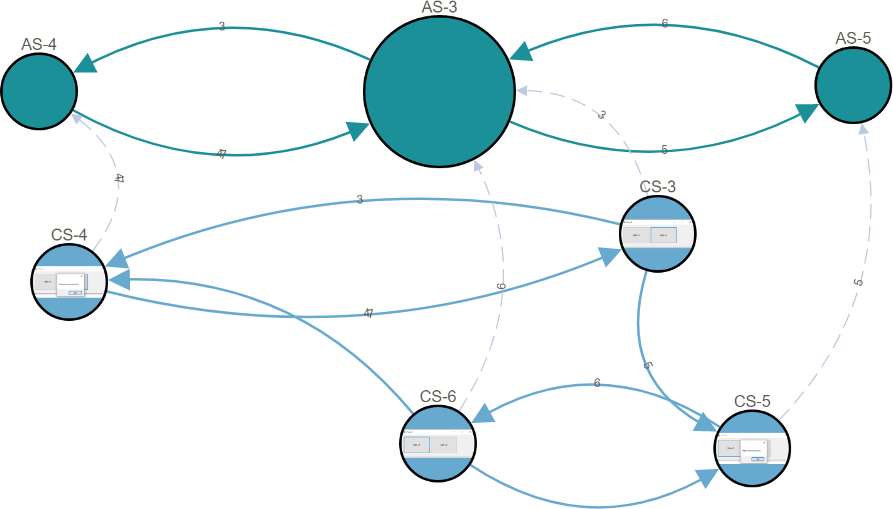
\includegraphics[scale=0.38]{pics/state-model.png}
\captionof{figure}{an inferred model in the visualisation application}\label{fig:state-model}
\endgroup

In figure \ref{fig:state-model} two models can be observed. The first model, indicated by the AS text, shows the abstract model. The second, indicated by the CS text, shows the concrete GUI states. 

\subsubsection{Concrete model}
The concrete model contains all the data that could be retrieved from the GUI. The identification key uses a hash calculated over all the properties. Aside from the widget's properties, the concrete models also contain a screenshot of the GUI for each state \cite{thesisMulders}.

Figure \ref{fig:concrete-node} shows an example of a node in the concrete model. Upon selecting a node, the properties of the node show, including the screenshot taken during the test. The grey dotted line, indicated with the letter 'a', shows the connection with the abstract node, see section \ref{abstract-model} and figure \ref{fig:abstract-model} for more details. The two outgoing edges, indicated with the letter 'b', shows the two actions available in this state. The incoming edge, indicated with the letter 'c', shows how the state was reached. 

\bigskip
\begingroup
\captionsetup{type=figure}
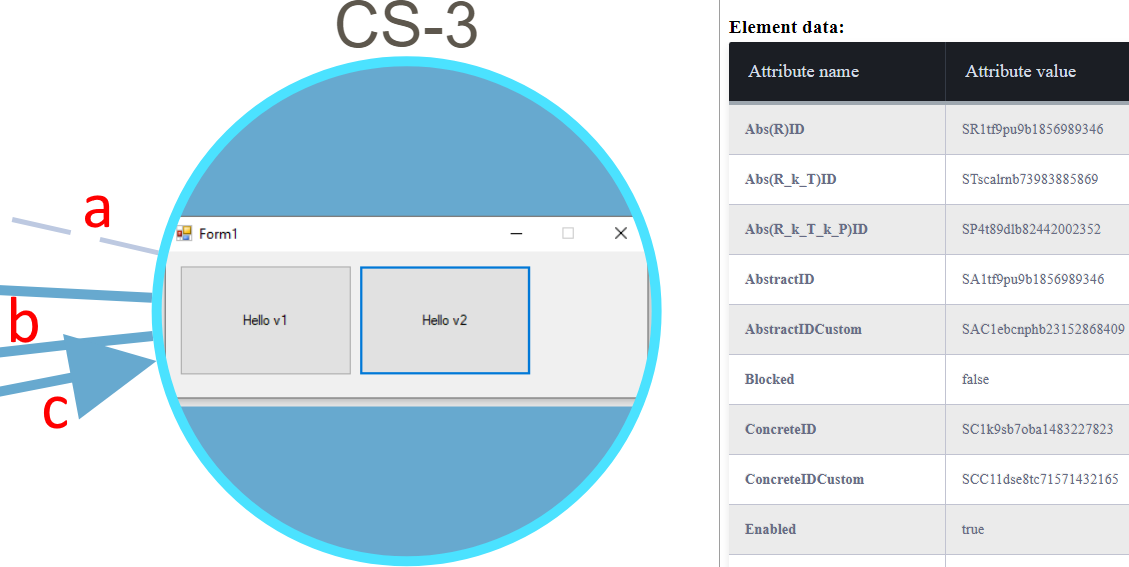
\includegraphics[scale=0.5]{pics/concrete-model.png}
\captionof{figure}{A node from the concrete model}\label{fig:concrete-node}
\endgroup

\newpage
\subsubsection{Abstract model} \label{abstract-model}
Since the concrete models containing all the data from a GUI-state, they can become quite large.  Therefore an abstraction model is made \cite{thesisMulders}. Figure \ref{fig:abstract-model} shows an example of such a abstract node. The grey lines (from CS-3, CS-6 to AS-3) indicates which concrete state is abstracted. The properties of the abstract node are displayed, what the identifier is and which concrete state(s) it represents.

\bigskip
\begingroup
\captionsetup{type=figure}
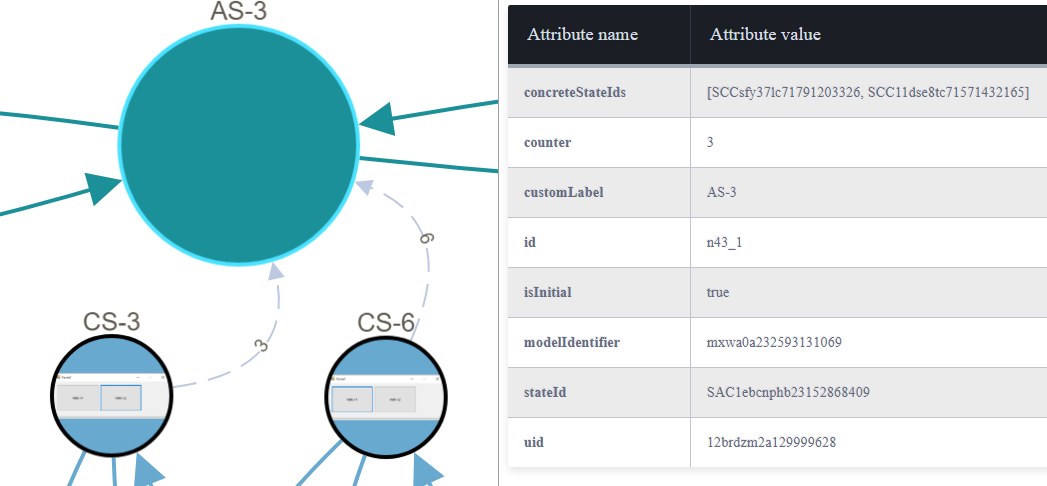
\includegraphics[scale=0.5]{pics/abstract-model.png}
\captionof{figure}{A node from the abstract model}\label{fig:abstract-model}
\endgroup

\subsubsection{State identifiers} \label{state-identifiers}
Every state must have a unique id for identification. The identifier is calculated with the data from the widget tree. 

TESTAR uses a hashing algorithm that works as follows: the widgets' properties are concatenated and hashed. The outcome will be used as the identifier for a widget. The hashes from the widget in the widget tree are then combined and hashed to create an identifier for the GUI state \cite{VosAho2021}. The TESTAR's algorithm is similar to how a Merkle tree works, more information can be found at section \ref{merkle-tree}.

To identify the state (and actions), TESTAR calculates two state identifiers; an abstract and concrete state identifier. For the concrete state identifier, all the properties of a widget are used. For the abstract identifier, a subset of the properties is used. It is configurable which properties are used for the abstract identifier. By default the properties \textit{role}, \textit{title}, \textit{position} and \textit{enabled} are utilised \cite{VosAho2021, thesisMulders}.

When running TESTAR, it is possible to configure which widget properties should be used for the abstract state identifier. Figure \ref{fig:advance} shows the selection dialogue in which the user can select the properties for the abstract identifier.

\subsection{Merkle tree} \label{merkle-tree}
A Merkle tree is a hash tree data structure where a hash can identify each vertex. \cite{merkle-tree} The cryptographic hash is calculated by taking the hashes of the descendant vertices, combining them, and calculating a new hash from the combination. 

As written in the previous section (\ref{state-identifiers}), TESTAR's way of calculating the identification id for a widget or a GUI state is similar to that of the Merkle tree vertex. The hashed id for a widget is based on the hashed property values. Figure \ref{fig:merkle-tree} shows an example of a Merkle tree about how the GUI state identification id is calculated. The corresponding widget tree (Figure \ref{fig:widget-tree}), where the Merkle tree is based, is shown in the top right corner.

Although a Merkle tree usually is a binary tree \cite{merkle-tree}, having more than two descendant vertices is not considered a problem since the same Merkle-tree principle can be applied.

\bigskip
\begingroup
\captionsetup{type=figure}
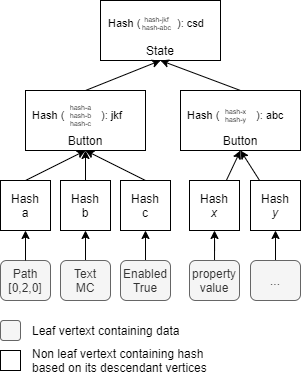
\includegraphics[scale=0.8]{pics/merkle-tree-example.png}
\captionof{figure}{An short Merkle tree example based on a widget tree}\label{fig:merkle-tree}
\endgroup

\subsubsection{How is an inferred model created?}
This research focuses itself on the outcome of the obtain step as illustrated in figure \ref{fig:obtain-state-graph}, which is the top right part of figure \ref{fig:testar-test-cycle}.

\bigskip
\begingroup
\captionsetup{type=figure}
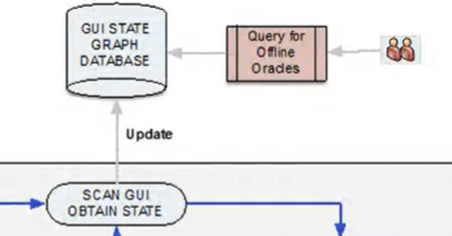
\includegraphics[scale=0.4]{pics/obtain-state-graph.png}
\captionof{figure}{The focus of this research proposal \cite{testar-presentation}}\label{fig:obtain-state-graph}
\endgroup

Generating the inferred model starts when TESTAR start testing the SUT. After an action has been executed successfully, the state of the GUI is sent to the inferred model module. When the state is reached without action, it is marked as the initial state. 

The inferred model module generates the abstract and concrete state's and saves those in the model. The model is persisted in the OrientDb database. At last, a deterministic model check is being performed and saved \cite{testar-code}.

\subsection{State model difference}
The \verb|StateModel.Difference| package, added by Pastor Ricós\cite{stateDiff}, offers a proof of concept for calculating differences between the inferred state models. For the comparison, the \verb|abstractStateId| is used. 

Pastor Ricós difference algorithm\cite{stateDiff} outputs two classification of changes between two models: added and removed state. Let $A$ be a set of \verb|abstractStateId|s of version 1 of the SUT, and let $B$ be a set of \verb|abstractStateId|s of version 2 of the SUT. The removed states can be written as
\[A-B = \lbrace x | x \in A \wedge x \notin B \rbrace\]
the states that are added can be written as
\[B-A = \lbrace x | x \in B \wedge x \notin A \rbrace\]

\begingroup
\captionsetup{type=figure}
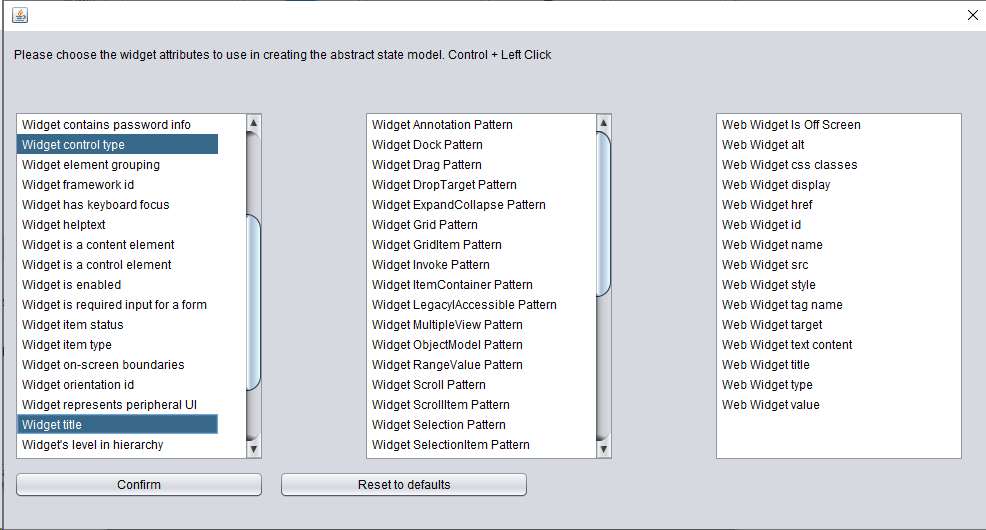
\includegraphics[scale=0.5]{pics/attributes-state-model.png}
\captionof{figure}{Select widgets attributes for the abstractStateId}\label{fig:advance}
\endgroup

Using the \verb|abstractStateId| is excellent for the proof of concept and preliminary change detection, 
However, its boolean nature in which state exists or not can result in many 'false' changes. For example, when a widget is moved, the change detection should result in an altered state, not a removed and added state. 

Section \ref{state-identifiers} discussed how identifiers are generated, since the differences are calculated based on the \verb|abstractStateId| selecting the correct widget attributes is vital. Choosing too few attributes could result in conflicting differences like the same actions are removed and added. Choosing too many attributes could trigger a change in even the tiniest detail. Choosing the widget attributes can be done with the 'Advance' screen under the State model tab. See Figure \ref{fig:advance}.

For the research proposal, an experiment application is created; the two-buttons app. With the two-buttons app, it was possible to experiment with various TESTAR settings. The application is shown in figures \ref{fig:exp-v1}, \ref{fig:exp-v2} and \ref{fig:exp-v3}. As one can observe, the differences between version 1 and version 2 are the added button with the label 'Hello v2' and between version 2 and 3 the buttons' colour and position. 

\begin{tabularx}{\textwidth}{@{} 
   >{\raggedright\arraybackslash}X
   >{\raggedright\arraybackslash}X  }
    \begingroup
    \captionsetup{type=figure}
    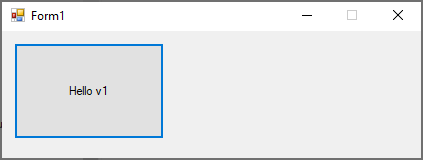
\includegraphics[scale=0.60]{pics/exp-v1.png}
    \captionof{figure}{Version 1 of the experiment application}\label{fig:exp-v1}
    \endgroup
    &
    \begingroup
    \captionsetup{type=figure}
    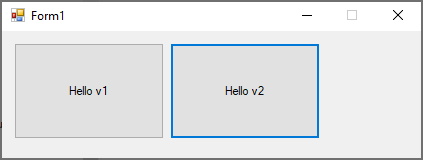
\includegraphics[scale=0.60]{pics/exp-v2.png}
    \captionof{figure}{Version 2 of the experiment application}\label{fig:exp-v2}
    \endgroup
    
    \\
    
    \begingroup
    \captionsetup{type=figure}
    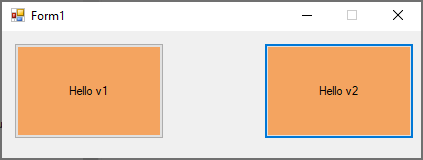
\includegraphics[scale=0.6]{pics/exp-v3.png}
    \captionof{figure}{Version 3 of the experiment application}\label{fig:exp-v3}
    \endgroup
\end{tabularx}


However, a different result is displayed when using 'widget title' and 'widget control type' as widget attributes for the abstract states. Namely, the button with the label 'Hello v1' is removed between the first two versions. The buttons labelled 'Hello v1' and 'Hello v2' are added. Between versions 2 and 3, no differences are observed.

This change difference outcome can be explained by the way the proof of concept is working. The widget tree of version 1 contains one button, whereas the widget tree of version 2 contains two buttons. Therefore both the abstract and the concrete identifiers are different for both widget trees. The proof of concept change detection checks whether the abstract identifier of version 1 can be found in version 2, which it cannot, so the state is marked as removed. The state of version 2 can likewise not be found in version 1 so that state is marked as new.

The chosen widget attributes explain the absence of changes between versions 2 and 3. Neither the title nor the control type has changed. Since those attributes were used for the abstract identifier, TESTAR did not detect a change. 

In section (\ref{research-questions}), the research questions are discussed. Of course, one of the questions will investigate how the change detection algorithm must be implemented. The findings of the two-button app should be considered, and the experiment should be adapted to contain different changes to test on. 

%\newpage
\subsection{TESTAR in containers}
A recent master thesis by Slomp explains how TESTAR can be integrated into a \acrfull{ci} environment \cite{thesisSlomp}. Slomp introduced TESTAR into the world of Docker and container and integrated TESTAR into an Azure DevOps pipeline. A pipeline is a collection of steps that can automatically build, test and release software. A container bundles all the software, configuration files and libraries together so that an application can run \cite{ms-container}. 

When TESTAR is being run within the Azure DevOps pipeline, the TESTAR GUI is not shown. Running TESTAR is not a problem. However, to analyse the outcome of TESTAR, the users need to install TESTAR and have access to the OrientDb database location. 

By moving the code for change detection and visualisation into a stand-alone web application, the user can analyse the outcome on their browser. Since TESTAR is wrapped into a container, the stand-alone tool will also be wrapped to provide the same infrastructure. Nevertheless, it is up to the IT administrator how they deploy the TESTAR suite. 

Additionally, to the user's benefit, a TESTAR developer can also benefit from the application's separation. Changes to either the separate application or TESTAR can be made without being conflicting with the other. Each tool can focus on one goal, while TESTAR can focus on testing GUI applications. 